% File name: Reports/First_Int_Report.tex
% First Interim Report for GF2 Software project. Details intro and
% general approach, teamwork planning, EBNF for syntax, informal
% description of semantics; error handling and example definition
% files and corresponding logic circuits
% Author: James Glanville, George Aryris and Andy Holt
% Date: Wed 15 May 2013 16:51

\documentclass[a4paper,11pt]{article}  % Standard document class
\usepackage[english]{babel}            % Set document language
\usepackage{fullpage}                  % Set up page for small margins etc

\usepackage{graphicx}                  % For including images in document
%\usepackage{placeins}                  % Allows use of \FloatBarrier
% to avoid images or tables
% moving into next section
%\usepackage{subfig}                    % For subfigures...

\usepackage{amsmath}                   % For improving maths/formula typesetting
%\usepackage{tabularx}                  % Table changing package

%\usepackage{algpseudocode}             % For producing algorithms/flowcharts

\usepackage{listings}                  % For including source code in document
\lstset{
  basicstyle = \small
}

% Provide command for scientific notation
\providecommand{\e}[1]{\ensuremath{\times10^{#1}}}
\providecommand{\degrees}{\ensuremath{^{\circ}}}

% Define title here:
\title{Project GF2: Software\\ First Interim Report\\ Software Design
  Team 1}
\author{George Ayris\\ gdwa2\\ Emmanuel \and James Glanville\\
jg597\\ Emmanuel \and Andrew Holt\\ ah635\\ Emmanuel}
\date{21 May 2013}

\begin{document}

% generate title
\maketitle

\section{Introduction}

This project requires the development of a logic simulation program,
implemented in C++. When completed, the application will read a
definition file containing a list of devices and the connections
between them. It will then graphically display the values of specified
monitor points in the circuit as the simulation is run. Some legacy
code has been provided, but lacks a scanner, parser and GUI which will
be developed in this project.

\subsection{Teamwork Planning}

The GUI development requires learning and reference to the wxWidgets
and OpenGL packages, so makes sense for one team member to focus
efforts here. The scanner and parser will require robust coding and
testing, so it was decided to combine the two as a peer programming
project to allow implementation and testing to be carried out by
different team members.

The work is to be distributed as follows: Andrew will code the GUI,
and James and George will write and test the scanner and parser. The
time frame for the development is that the software should be designed
by the end of Tuesday 21$^{\mathrm{st}}$ May; implemented and unit
tested by Tuesday 28$^{\mathrm{th}}$; allowing time for system
integration and testing by 11.00am on Friday 31$^{\mathrm{st}}$ May.

\section{Syntax Specification}

The syntax for the circuit definition files was defined and described
using the following EBNF grammar:
\begin{lstlisting}
DEFINITION = `{' DEVICES INIT CONNECTIONS MONITORS `}'

DEVICES =  `DEVICES' `{' device {device} `}'
device = devicename `=' devicetype [ `(' digit {digit} `)' ] `;'
devicename = letter {letter | digit}
devicetype = `AND' | `NAND' | `OR' | `NOR' | `XOR' | `DTYPE' | `CLK' | `SW'

INIT = `INIT' `{' {init} `}'
init = devicename `=' digit{digit} `;'

CONNECTIONS = `CONNECTIONS' `{' connection {connection} `}'
connection = input `<=' output `;'
input = letter {letter|digit} [`.'letter|digit{letter|digit}]
output = letter {letter|digit} [`.'letter|digit{letter|digit}]

MONITORS = `MONITORS' `{' monitor {monitor} `}'
monitor = monitorname `<=' output `;'
monitorname = letter{letter|digit}
\end{lstlisting}

\section{Semantics Specification}

The following set of semantic descriptions was created to describe the
semantics.
\begin{itemize}
  \item A logic circuit is defined in a file that opens with ``\{'' and
      closes with ``\}''.
  \item Each file has four sections: ``\texttt{DEVICES}'',
    ``\texttt{CONNECTIONS}'', ``\texttt{MONITORS}'' and
    ``\texttt{INIT}''. Each section starts with the section name
    followed by a ``\{'' and terminates with a ``\}''.
  \item Within ``\texttt{DEVICES}'' there must be at least one
    device.
 \item All names and keywords are case-insensitive,
   i.e. \texttt{GATE1.O} and \texttt{gate1.o} are the same, and must
   be unique. 
  \item A device is defined by ``\texttt{devicename =
      devicetype(N);}'', where the parentheses and parameter are only
    required for certain device types.
  \item A device name is alphanumeric and must begin with a letter.
  \item If the device has a variable number of inputs then the number
    required for the device must be specified in parentheses after the
    device type. The number of inputs specified must lie within the
    allowable range for that device type.
  \item Within ``\texttt{CONNECTIONS}'' every input (of defined
    devices) must be connected to a single device output.
  \item A connection is defined as ``\texttt{input <=
      output;}''. Where input must correspond to a defined device
    input and output to a defined device output.
  \item An input is specified by
    ``\texttt{devicename.inputidentifier}''.
  \item An output is specified by
    ``\texttt{devicename.outputidentifier}''.
  \item The clock, switch and gate outputs are accessed with
    ``\texttt{.o}''.
  \item The gate inputs are accessed with ``\texttt{.n}'' where
    \texttt{n} is 1 or 2 for XOR gates and 1-16 for all the other
    gates.
  \item The \texttt{DTYPE} inputs are accessed with ``\texttt{.d}'',
    ``\texttt{.c}'', ``\texttt{.s}'' and ``\texttt{.r}'', which
    represent \texttt{DATA}, \texttt{CLK}, \texttt{SET} and
    \texttt{RESET} (rather than \texttt{CLEAR} to avoid confusion with
    \texttt{CLK}).
  \item The \texttt{DTYPE} outputs are accessed with ``\texttt{.o}''
    and ``\texttt{.no}'' for normal output (\texttt{Q}) and inverting
    output (\texttt{QBAR}).
  \item Within ``\texttt{MONITORS}'' at least one monitor must be
    defined.
  \item A monitor is defined as ``\texttt{monitorname <= output}'',
    where outputs are specified as above.
  \item A monitorname is alphanumeric and must begin with a letter.
  \item Within ``\texttt{INIT}'' all defined switches and clocks must
    have an initialisation.
  \item Clocks are initialised with a period of \texttt{n} simulation
    cycles, where \texttt{n} is a positive integer.
  \item Switches are initialised with a state that is either 1 or 0,
    where 1 is a logic high state on the output and 0 is a logic low
    state.
  \item Initialisation is done by ``\texttt{devicename = value;}'', where
    devicename is an already defined device and value is legal for the
    device type.
  \item Comments in the definition file are defined as any data
    between an opening ``\texttt{/*}'' and a closing ``\texttt{*/}''. Comments may be
    nested.
\end{itemize}

\section{Error Handling}

The scanner will pass symbols to the parser, one at a time. The
symbols will also be stored in a private list in the scanner
class. The parser will check that the syntax and semantic rules are
followed as each symbol comes in from the scanner. If an error is
found, the parser will pass an error message to the scanner. The
scanner will know which symbol was last passed, and hence which
generated the error. The line will then be printed with a carat
(\verb+^+) pointing at the offending symbol, along with the error
message that will give a brief description of what is wrong, such as
``\texttt{expected `)' instead of `;'}'', so as to inform the user how
to fix the definition file.

When an error is found, the system will not continue to process the
file beyond the end of that line, as one error is likely to cause
further errors. This will allow just the first error to be shown,
allowing easy debugging by the user, as they know exactly where the
error has occurred without being distracted by other errors that
resulted. The downside of this is that only one error will be shown at
a time, so independent errors cannot be debugged at the same time. 

The parser class is directly translated from the EBNF, and when the
parsing routine encounters a symbol that does not correlate with the
EBNF then an error will be reported. The EBNF specifies
semi colons at the end of most lines, so parsing can stop as soon as
it reaches the next semi colon.

Some of the semantic errors will be checked on a line by line basis,
such as ensuring that the parameters in the expression are legal and
defined. Others will require waiting until the section is completed,
such as ensuring that all device inputs have a specified
connection. This will be checked when the closing brace (\verb+}+)
denoting the end of the section is parsed.

\section{Example Circuits and Definition Files}

The following two examples show how to define logic circuits using our
definition language. Both are common logic applications, the first is
making a more complex logic device from the easiest to manufacture
device, the NAND gate. The other shows how to define a common
sequential logic, a 3 but Gray Code counter, implemented in D-type
bistables.

\subsection{XOR Circuit Composed of NAND Gates}

The XOR circuit is shown in figure \ref{fig:xornand}. The
specification file is shown below.

\begin{figure}[!h]
  \begin{center}
    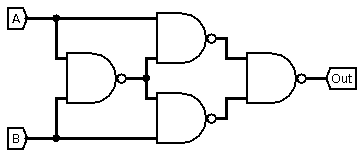
\includegraphics[width=0.8\textwidth]{XORfromNAND.png}
  \end{center}
  \caption{XOR circuit composed of NAND gates.}
  \label{fig:xornand}
\end{figure}

\begin{lstlisting}
{
  DEVICES
  {
    N1 = NAND(2);
    N2 = NAND(2);
    N3 = NAND(2);
    N4 = NAND(2);
    SWA = SW;
    SWB = SW;
  }

   INIT
   {
     SWA.O=1;
     SWB.O=0;
   }

   CONNECTIONS
   {
     N1.1 <= A.O;
     N1.2 <= B.O;
     N2.1 <= A.O;
     N2.2 <= N1.O;
     N3.1 <= N1.O;
     N3.2 <= B.O;
     N4.1 <= N2.O;
     N4.2 <= N3.O;
   }

   MONITORS
   {
     OUT1 <= N4.O;
   }
 }

\end{lstlisting}

\subsection{3-bit Gray Code Counter}

The 3-bit Gray code counter is shown in figure \ref{fig:3bitgray}, and
specified below.

\begin{figure}[!h]
  \begin{center}
    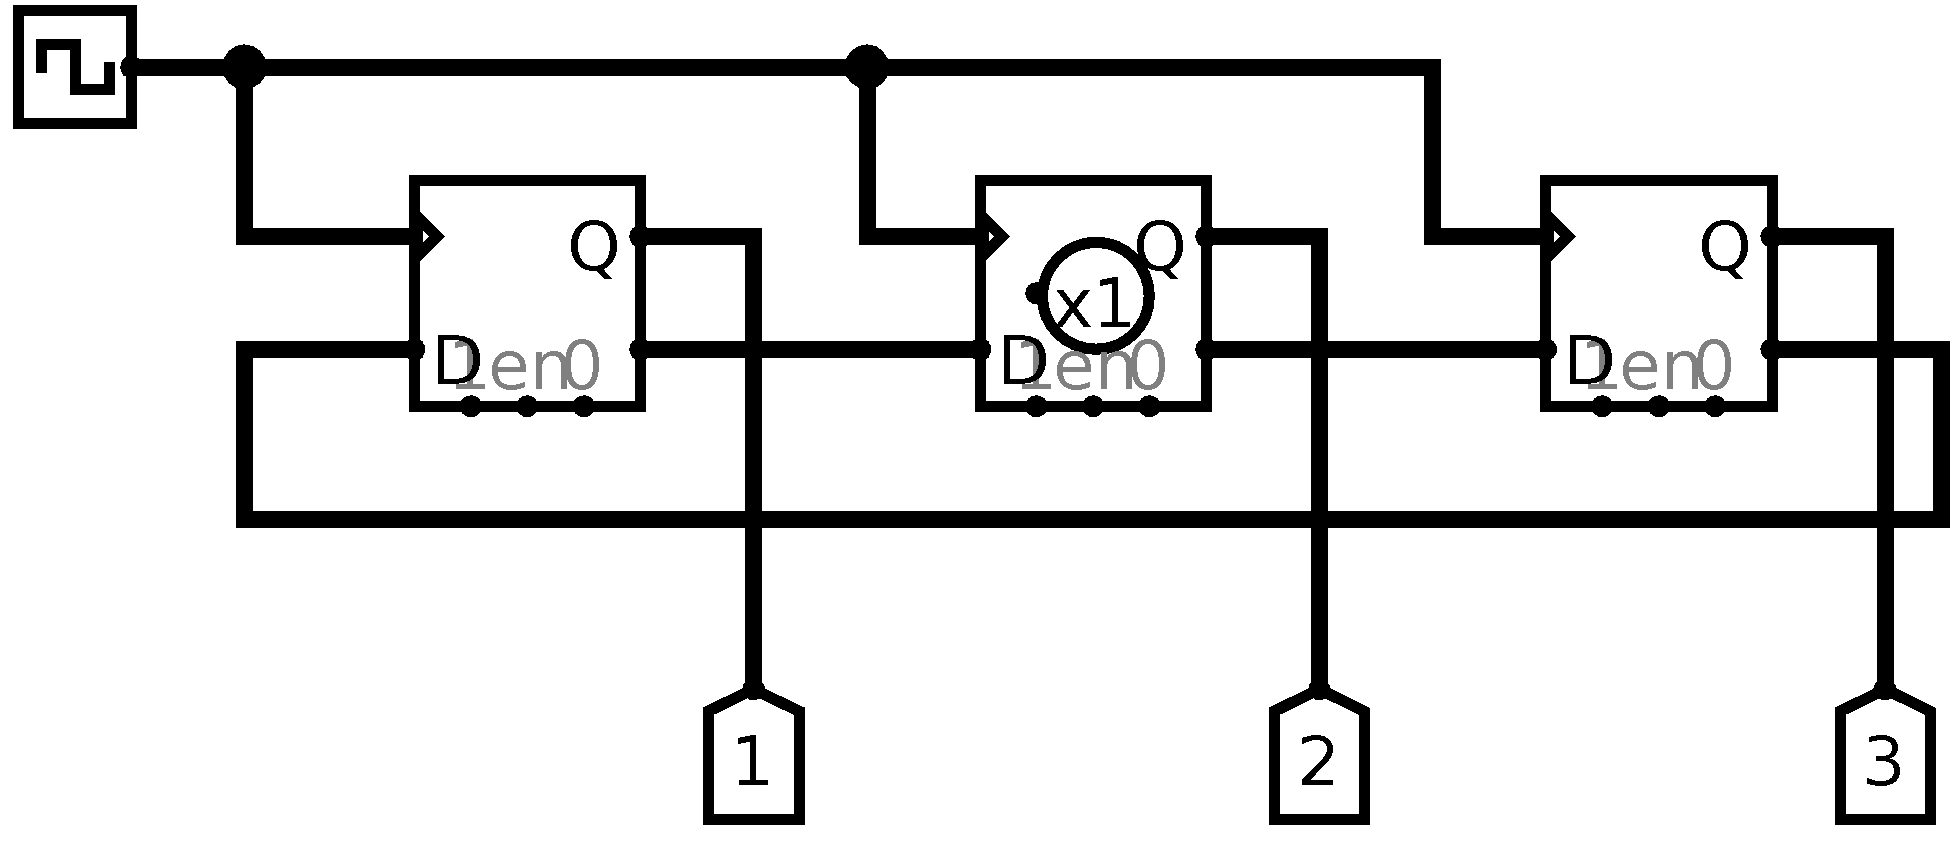
\includegraphics[width=0.8\textwidth]{3bitGrayCounter.png}
  \end{center}
  \caption{3 bit Gray code counter from D-type bistables}
  \label{fig:3bitgray}
\end{figure}

\begin{lstlisting}
{
  DEVICES
  {
    D1 = DTYPE;
    D2 = DTYPE;
    D3 = DTYPE;
    CLK1 = CLK;
  }

  INIT
  {
    CLK1 = 1;
  }
  
  CONNECTIONS
  {
    D1.C <= CLK1.O;
    D2.C <= CLK1.O;
    D3.C <= CLK1.O;
    D1.D   <= D3.NO;
    D2.D   <= D1.NO;
    D3.D   <= D2.NO;
  }
  
  MONITORS
  {
    OUT1 <= D1.O;
    OUT2 <= D2.O;
    OUT3 <= D3.O;
  }
}
\end{lstlisting}

\end{document}